\documentclass[10pt,aspectratio=169]{beamer}
\usetheme[progressbar=frametitle,numbering=fraction]{metropolis}
\usepackage[utf8]{inputenc}
\usepackage[T1]{fontenc}
\usepackage{booktabs}
\usepackage{array}
\newcolumntype{L}[1]{>{\raggedright\arraybackslash}p{#1}}
\usepackage{tikz}
\usetikzlibrary{arrows.meta,positioning,shapes.geometric,fit,backgrounds}
\usepackage{pgfplots}
\pgfplotsset{compat=1.17}
\usepackage{listings}

% ---------------------------------------------------------------------------
\definecolor{accent}{HTML}{1F6FB2}
\definecolor{old}{HTML}{B2452E}
\definecolor{new}{HTML}{2E7D4F}
\definecolor{soft}{HTML}{EEF3F8}
\setbeamercolor{frametitle}{bg=accent}
\setbeamercolor{progress bar}{fg=accent}
\setbeamercolor{alerted text}{fg=old}
\setbeamercolor{example text}{fg=new}

\lstset{basicstyle=\ttfamily\scriptsize, columns=fullflexible, keepspaces=true,
        backgroundcolor=\color{soft}, frame=none, xleftmargin=4pt, xrightmargin=4pt,
        showstringspaces=false, commentstyle=\color{gray}, upquote=true}
\newcommand{\code}[1]{\texttt{\small #1}}

\title{GENIE for FASER}
\subtitle{A native build without the ATLAS container,\\ and what changes from 3.04 to 3.06}
\author{André Rubbia}
\institute{ETH Zürich, IPA}
\date{October 2026}

\begin{document}

\maketitle

% ---------------------------------------------------------------------------
\begin{frame}{Outline}
  \begin{enumerate}
    \item Why the old recipe needed the ATLAS container
    \item The new build: one repository, two scripts
    \item Pitfalls solved along the way (macOS / modern ROOT)
    \item GENIE 3.04 (FASER fork) $\rightarrow$ 3.06.02: what changed
    \item Validation: event rate and a geometry-unit bug
    \item Next steps
  \end{enumerate}
\end{frame}

% ===========================================================================
\section{The old recipe}

\begin{frame}{How 3.04 was built}
  \begin{columns}[T]
    \column{0.55\textwidth}
    \begin{itemize}
      \item \code{setupATLAS -c centos7}: Apptainer container with CentOS 7
      \item \code{asetup Athena,22.0.49}: only to get compilers and libraries from CVMFS
            (gcc 11, ROOT 6.24, Pythia6, LHAPDF, GSL, \dots)
      \item TPythia6 built as an \emph{Athena/Calypso} CMake project
      \item GENIE itself: plain \code{./configure \&\& make}
    \end{itemize}
    \column{0.42\textwidth}
    \begin{alertblock}{Problems}
      \begin{itemize}\small
        \item CentOS 7 is end-of-life: the container exists only to run old binaries
        \item mixed gcc8 and gcc11 libraries on one \code{LD\_LIBRARY\_PATH}
        \item broken Pythia6 link line in \code{Make.include}
        \item not usable on a Mac
        \item no easy path to move to Pythia8
      \end{itemize}
    \end{alertblock}
  \end{columns}
  \vfill
  \begin{exampleblock}{Key point}
    GENIE contains no ATLAS code. Athena was only a convenient way to get a software stack.
  \end{exampleblock}
\end{frame}

\begin{frame}{What GENIE actually needs}
  \centering
  \begin{tabular}{@{}lll@{}}
    \toprule
    Dependency & Role & Source in the new build \\
    \midrule
    ROOT (with Geom) & I/O, geometry (TGeo), maths & conda-forge / LCG view \\
    Pythia 6.4.28 & hadronization, decays & built from \code{alisw/pythia6} \\
    TPythia6 (\code{libEGPythia6}) & ROOT interface to Pythia6 & built here (plain CMake) \\
    LHAPDF 6 & PDFs & conda-forge / LCG \\
    GSL, libxml2, log4cpp & numerics, config, logging & conda-forge / LCG \\
    \midrule
    \emph{optional:} APFEL 3.0.6 & HEDIS structure functions & \code{WITH\_APFEL=1} \\
    \emph{optional:} Pythia 8 & Pythia8 hadronization & \code{WITH\_PYTHIA8=1} \\
    \bottomrule
  \end{tabular}
  \vspace{1em}

  \small TPythia6 was removed from ROOT in 6.32, so it is compiled from the old ROOT sources.\\
  APFEL is off by default: the FASER splines and tunes do not use HEDIS.
\end{frame}

% ===========================================================================
\section{The new build}

\begin{frame}{Overview}
  \centering
  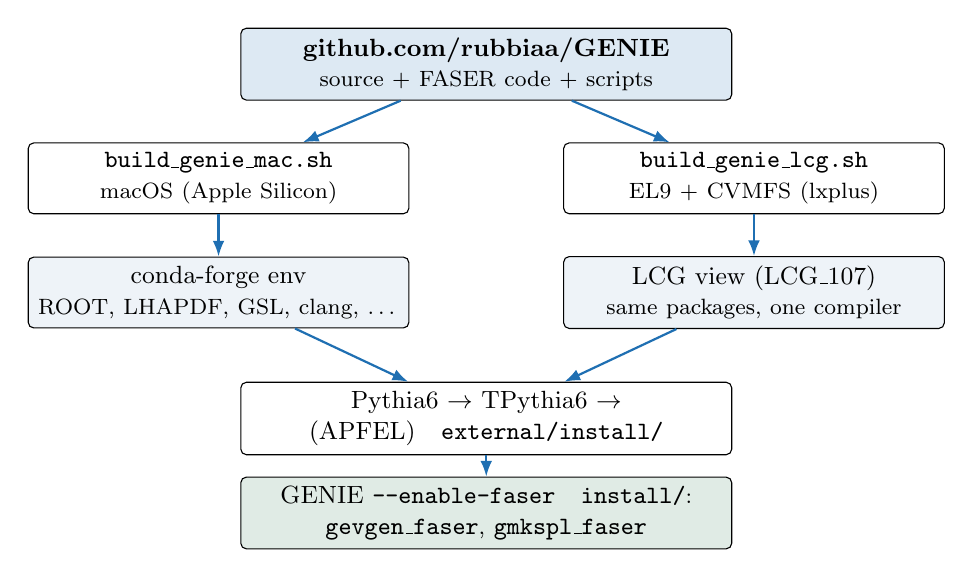
\begin{tikzpicture}[
      box/.style={draw, rounded corners=2pt, align=center, font=\small, minimum height=9mm, fill=white, text width=46mm},
      dep/.style={box, fill=soft},
      arr/.style={-{Latex[length=2mm]}, thick, accent}]
    \node[box, fill=accent!15, text width=60mm] (repo) at (0,0) {\textbf{github.com/rubbiaa/GENIE}\\ \footnotesize source + FASER code + scripts};
    \node[box] (mac) at (-3.4,-1.45) {\code{build\_genie\_mac.sh}\\ \footnotesize macOS (Apple Silicon)};
    \node[box] (lcg) at ( 3.4,-1.45) {\code{build\_genie\_lcg.sh}\\ \footnotesize EL9 + CVMFS (lxplus)};
    \node[dep] (conda) at (-3.4,-2.9) {conda-forge env\\ \footnotesize ROOT, LHAPDF, GSL, clang, \dots};
    \node[dep] (view)  at ( 3.4,-2.9) {LCG view (LCG\_107)\\ \footnotesize same packages, one compiler};
    \node[box, text width=60mm] (ext) at (0,-4.5) {Pythia6 $\rightarrow$ TPythia6 $\rightarrow$ (APFEL)\quad \footnotesize\code{external/install/}};
    \node[box, fill=new!15, text width=60mm] (genie) at (0,-5.7) {GENIE \code{-{}-enable-faser}\quad \footnotesize\code{install/}: \code{gevgen\_faser}, \code{gmkspl\_faser}};
    \draw[arr] (repo) -- (mac);  \draw[arr] (repo) -- (lcg);
    \draw[arr] (mac) -- (conda); \draw[arr] (lcg) -- (view);
    \draw[arr] (conda) -- (ext); \draw[arr] (view) -- (ext);
    \draw[arr] (ext) -- (genie);
  \end{tikzpicture}

  \vspace{-2pt}\small No container, no Athena, no \code{asetup}. The same scripts work on both platforms.
\end{frame}

\begin{frame}[fragile]{Repository = work directory}
  \begin{columns}[T]
    \column{0.52\textwidth}
\begin{lstlisting}
GENIE3.06/                  <- git repository
|-- README.md
|-- GENIE_3.04_vs_3.06.md
|-- setup_mac.sh   build_genie_mac.sh
|-- setup_lcg.sh   build_genie_lcg.sh
|-- GenieGenerator/         <- GENIE 3.06.02 + FASER
|   |-- src/  config/  data/
|   |-- faser/   (geometries, fluxes, scripts)
|   |   |-- TPythia6_standalone/
|   |   `-- build/external/  (patch, Pythia6 CMake)
|-- install/          \
|-- external/          |  created by the
|-- build/             |  build, ignored by git
|-- faser_xsec/        |
`-- run/              /
\end{lstlisting}
    \column{0.44\textwidth}
    \begin{itemize}\small
      \item Full GENIE history kept (7\,962 commits), FASER work on top
      \item Build products, downloads, splines and event files are \emph{git-ignored}
      \item Large Kling 2023 flux ntuples ($\le 575$\,MB) not in git: regenerated with
            \code{getRawFluxes.sh} + \code{convertAllFluxes.sh}
      \item Scripts find the source tree and work directory automatically
    \end{itemize}
  \end{columns}
\end{frame}

\begin{frame}[fragile]{Building on a Mac}
\begin{lstlisting}
git clone https://github.com/rubbiaa/GENIE.git GENIE3.06
cd GENIE3.06
./build_genie_mac.sh          # first time ~20 min
source setup_mac.sh           # every new terminal (zsh or bash)
\end{lstlisting}
  \vspace{0.5em}
  What the script does:
  \begin{enumerate}\small
    \item installs a private Miniforge in \code{\textasciitilde/miniforge3} (does not touch \code{.zshrc} or an existing Anaconda)
    \item creates the \code{genie} env: \code{root lhapdf gsl libxml2 log4cpp cmake make clang gfortran}
    \item builds Pythia 6.4.28 and TPythia6 into \code{external/install/}
    \item patches \code{Make.include} for Apple Silicon and the conda compilers (idempotent)
    \item \code{./configure -{}-enable-faser \dots}, \code{make}, \code{make install}
  \end{enumerate}
  \small Options: \code{WITH\_PYTHIA8=1}, \code{WITH\_APFEL=1}, \code{NJ=<jobs>}.
\end{frame}

\begin{frame}[fragile]{Building on lxplus (EL9 + CVMFS)}
\begin{lstlisting}
git clone https://github.com/rubbiaa/GENIE.git GENIE3.06 && cd GENIE3.06
./build_genie_lcg.sh                      # LCG_107, x86_64-el9-gcc13-opt
LCG_VERSION=LCG_105 ./build_genie_lcg.sh  # any other release
source setup_lcg.sh
\end{lstlisting}
  \vspace{0.5em}
  \begin{itemize}\small
    \item One LCG view provides ROOT, Pythia6, LHAPDF, GSL, log4cpp and libxml2,
          all built with the same compiler
    \item \code{setup\_lcg.sh} replaces \code{ATLAS\_container.sh}, \code{.asetup.save},
          \code{kk} and \code{setupGenerator.sh}
    \item Only TPythia6 and GENIE are compiled locally
  \end{itemize}
\end{frame}

% ===========================================================================
\section{Pitfalls solved}

\begin{frame}{Problems found and fixed (all automatic in the scripts)}
  \footnotesize
  \begin{tabular}{@{}L{0.31\textwidth}L{0.64\textwidth}@{}}
    \toprule
    Symptom & Cause $\rightarrow$ fix \\
    \midrule
    conda solve never finishes & old Anaconda classic solver $\rightarrow$ private Miniforge with \code{mamba} \\
    \code{expected ')'} in \code{<charconv>} & clang 18 with libc++ 20 headers (ROOT pin) $\rightarrow$ match clang to the headers \\
    \code{undeclared identifier NAN} & macOS 27 SDK takes \code{NAN} from \code{<float.h>}; strict \code{-std=c++20} hides it $\rightarrow$ \code{-std=gnu++20} \\
    libc++ ``feature unavailable'' & conda targets macOS 11 $\rightarrow$ \code{-D\_LIBCPP\_DISABLE\_AVAILABILITY} \\
    \code{rootcling} fails & dictionary step does not see \code{CXXFLAGS} $\rightarrow$ flags also passed via the include options \\
    \code{-lPythia6}/\code{-lEGPythia6} not found & \code{make distclean} empties \code{install/} $\rightarrow$ externals in \code{external/install/}; library path added \\
    APFEL: \code{arm64-apple} unknown & 2013 \code{config.sub} $\rightarrow$ use \code{aarch64-apple-darwin} \\
    Apple Silicon flags & generic \code{macosx64} block (Xcode-10 era) $\rightarrow$ dedicated \code{macosxarm64} block \\
    \bottomrule
  \end{tabular}
\end{frame}

% ===========================================================================
\section{3.04 $\rightarrow$ 3.06}

\begin{frame}{Where the versions sit}
  \centering
  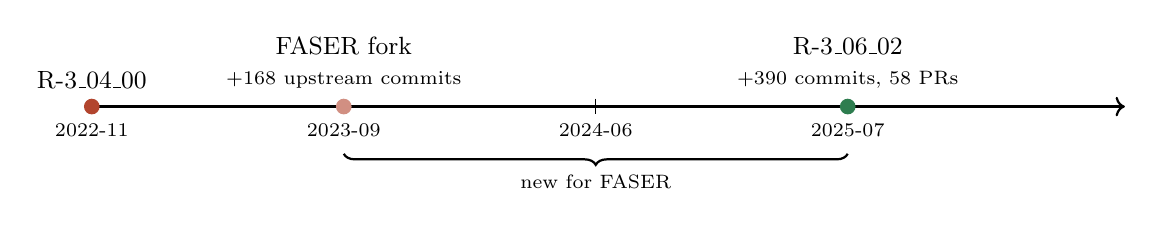
\begin{tikzpicture}[x=1.6cm]
    \draw[thick,->] (0,0) -- (8.2,0);
    \foreach \x/\l in {0/2022-11, 2/2023-09, 4/2024-06, 6/2025-07}{
      \draw (\x,0.1) -- (\x,-0.1) node[below,font=\scriptsize]{\l};}
    \node[circle,fill=old,inner sep=2pt,label={[font=\small,align=center]above:R-3\_04\_00}] at (0,0) {};
    \node[circle,fill=old!60,inner sep=2pt,label={[font=\small,align=center]above:FASER fork\\\scriptsize +168 upstream commits}] at (2,0) {};
    \node[circle,fill=new,inner sep=2pt,label={[font=\small,align=center]above:R-3\_06\_02\\\scriptsize +390 commits, 58 PRs}] at (6,0) {};
    \draw[decorate,decoration={brace,amplitude=4pt,mirror},thick] (2,-0.6) -- (6,-0.6)
       node[midway,below=4pt,font=\scriptsize]{new for FASER};
  \end{tikzpicture}
  \vspace{1em}
  \begin{itemize}
    \item \code{R-3\_06\_02} in the FASER GitLab is a plain mirror of the official release:
          \alert{no FASER code}
    \item Default tune unchanged: \code{G18\_02a\_00\_000}; its model configuration is identical
    \item About 1\,480 files differ upstream (configs, new models, data tables)
  \end{itemize}
\end{frame}

\begin{frame}{FASER code ported to 3.06}
  \footnotesize
  \begin{tabular}{@{}L{0.5\textwidth}L{0.43\textwidth}@{}}
    \toprule
    Item & Status \\
    \midrule
    \code{gevgen\_faser}, \code{gmkspl\_faser} & ported unchanged \\
    \code{FaserGMCJDriver}, \code{FaserROOTGeomAnalyzer} & ported; base interfaces unchanged \\
    \code{configure -{}-enable-faser}, \code{Apps/Makefile} & applied cleanly \\
    \code{GVLD-Emax} = \textbf{7\,TeV} (official: 1\,TeV) & re-applied \\
    \code{NaturalIsotopes::GetIsotopeData()} & re-added \\
    weighted-flux POT fix in \code{GSimpleNtpFlux} & \textbf{already upstream} \\
    tunes \code{F23\_00a}, \code{G25\_01a} & ported \\
    \code{faser/} (geometries, fluxes, scripts) & copied; big fluxes git-ignored \\
    TGeo length units (see validation) & \alert{new fix} \\
    \bottomrule
  \end{tabular}
  \vspace{0.6em}

  \small Not ported: the fork's broken Pythia6 lines in \code{Make.include}, which also removed the Pythia8 link block.
\end{frame}

\begin{frame}{Upstream changes relevant to FASER}
  \begin{columns}[T]
    \column{0.5\textwidth}
    \textbf{Pythia6 / Pythia8}
    \begin{itemize}\small
      \item Pythia6 now optional (\code{-{}-disable-pythia6})
      \item decayer: \code{PythiaDecayer} $\rightarrow$ \code{Pythia6Decayer2023}\\ (and \code{Pythia8Decayer2023})
      \item DIS charm: \code{AGCharm2019} $\rightarrow$ \code{AGCharmPythia6Hadro2023}\\ (same parameters)
      \item HEDIS hadronization: \code{LeptoHadPythia6/8}
      \item HE leptons: separate Pythia6/8 W-decay classes
    \end{itemize}
    \column{0.47\textwidth}
    \textbf{Other}
    \begin{itemize}\small
      \item memory-leak fixes (long productions)
      \item $G_F$, $\alpha$ configurable in \code{CommonParam.xml}
      \item build: Apple Silicon support, no \code{ROOTSYS} needed
    \end{itemize}
    \textbf{Not used by default}
    \begin{itemize}\small
      \item tunes \code{G24\_20i/j/k/l}, \code{N24\_20i}, \code{MK19\_00a}
      \item MK single-pion model, Z-expansion and MArun form factors, SuSAv2/CRPA updates
    \end{itemize}
  \end{columns}
  \vfill
  \small $\Rightarrow$ Expect small event-level differences in decays and charm hadronization: validate before production.
\end{frame}

% ===========================================================================
\section{Validation}

\begin{frame}{First comparison: 774 vs 40\,085 events}
  \small Same command, flux, geometry and (3.04) splines: \code{gevgen\_faser -l 1000} (1000\,fb$^{-1}$), FASERCal V10, Aki 2024 light flux.
  \begin{columns}[c]
    \column{0.56\textwidth}
    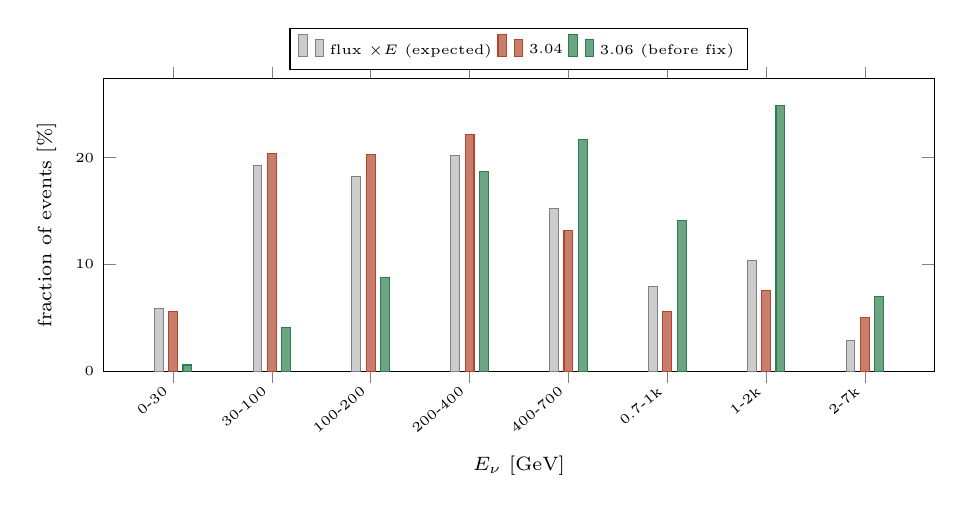
\begin{tikzpicture}
      \begin{axis}[ybar, width=\linewidth, height=5.3cm, bar width=3.2pt,
          ylabel={fraction of events [\%]}, ymin=0,
          symbolic x coords={0-30,30-100,100-200,200-400,400-700,0.7-1k,1-2k,2-7k},
          xtick=data, x tick label style={rotate=40,anchor=east,font=\tiny},
          xlabel={$E_\nu$ [GeV]}, xlabel style={font=\scriptsize}, ylabel style={font=\scriptsize},
          y tick label style={font=\tiny},
          legend style={font=\tiny, at={(0.5,1.03)}, anchor=south, legend columns=3}]
        \addplot[fill=gray!40, draw=gray] coordinates {(0-30,5.9) (30-100,19.3) (100-200,18.2) (200-400,20.2) (400-700,15.2) (0.7-1k,7.9) (1-2k,10.4) (2-7k,2.9)};
        \addplot[fill=old!70, draw=old] coordinates {(0-30,5.6) (30-100,20.4) (100-200,20.3) (200-400,22.2) (400-700,13.2) (0.7-1k,5.6) (1-2k,7.6) (2-7k,5.0)};
        \addplot[fill=new!70, draw=new] coordinates {(0-30,0.6) (30-100,4.1) (100-200,8.8) (200-400,18.7) (400-700,21.7) (0.7-1k,14.1) (1-2k,24.9) (2-7k,7.0)};
        \legend{flux $\times E$ (expected), 3.04, 3.06 (before fix)}
      \end{axis}
    \end{tikzpicture}
    \column{0.42\textwidth}
    \begin{itemize}\small
      \item 3.04 follows flux $\times\,\sigma \propto E$, as expected for DIS
      \item 3.06 deficit depends on energy: $\times 450$ below 30\,GeV, $\times 16$ above 1\,TeV
      \item Splines, flux code and FASER code were checked: \textbf{not} the cause
    \end{itemize}
  \end{columns}
\end{frame}

\begin{frame}[fragile]{Cause: TGeo length units}
  \centering\small
  \begin{tabular}{@{}lccc@{}}
    \toprule
    & 3.04 & 3.06 (before fix) & true geometry (GDML) \\
    \midrule
    vertex $x$ (5--95\%) & 0.4--1.2\,m & 0.04--0.14\,m & detector centred at 0.45\,m \\
    vertex $z$ (5--95\%) & 0.9--6.7\,m & 0.04--0.68\,m & target 0--2.9\,m, MDT at 6.1\,m \\
    \bottomrule
  \end{tabular}
  \vspace{0.6em}
  \begin{columns}[T]
    \column{0.52\textwidth}
    \begin{itemize}\small
      \item The FASER apps hard-wire geometry lengths in \textbf{mm}
      \item ROOT 6.16--6.24 (3.04 production): TGeo default \code{kG4Units} (mm) \checkmark
      \item ROOT $\geq$ 6.26 (6.40 here): default \code{kRootUnits} (cm)
      \item[$\Rightarrow$] detector 10$\times$ too small: shorter paths, and only the forward
            (high-energy) neutrinos hit it
    \end{itemize}
    \column{0.44\textwidth}
\begin{lstlisting}[language=C++]
// FaserROOTGeomAnalyzer::Load()
TGeoManager::LockDefaultUnits(false);
TGeoManager::SetDefaultUnits(
        TGeoManager::kG4Units);   // mm
TGeoManager::LockDefaultUnits(true);
TGeoManager::Import(filename);
\end{lstlisting}
    \begin{exampleblock}{Status}\small
      Fixed and committed. The rerun should give $\approx 40$k events, compatible with 3.04.
    \end{exampleblock}
  \end{columns}
\end{frame}

% ===========================================================================
\section{Next steps}

\begin{frame}{Next steps}
  \begin{enumerate}
    \item \textbf{Confirm the units fix:} rerun the 1000\,fb$^{-1}$ light and charm samples and compare
          with 3.04 (rates, $E_\nu$, targets, vertices)
    \item \textbf{Regenerate splines for 3.06} with \code{faser/Splines/}
          (free nucleons $\rightarrow$ nuclei, 6 flavours, up to 7\,TeV; $\sim$2--3 days on 16 cores)
    \item \textbf{Physics validation} of the rewritten decays and charm hadronization
          (charm and $\tau$ samples)
    \item \textbf{Optional:} Pythia8 hadronization (\code{WITH\_PYTHIA8=1}), then drop Pythia6
    \item \textbf{Share:} push \code{faser-R-3\_06\_02} back to the FASER GitLab
  \end{enumerate}
\end{frame}

\appendix
\begin{frame}[fragile]{Backup: command cheat sheet}
\begin{lstlisting}
# environment
source setup_mac.sh                      # or setup_lcg.sh on lxplus

# incremental rebuild after a code change
cd GenieGenerator && make -j && make install && cd ..

# event generation (FASERCal V10, Aki 2024 light flux, 1000 fb^-1)
gevgen_faser -l 1000.0 -r 0 -g $GENIE/faser/FASERCAL_V10.gdml \
   -f $GENIE/faser/Fluxes/Aki_2024/events_light_4x4.root --seed 2999833 \
   --cross-sections $GENIE_HOME/faser_xsec/faserSplines.7TeV.xml \
   -o fasercal.Aki2024.v10.light

# splines (run in GENIE3.06/splines_work, one flavour at a time)
source $GENIE/faser/Splines/calcSplinesN.sh;  wait
source $GENIE/faser/Splines/mergeSplinesN.sh
source $GENIE/faser/Splines/calcNuMuSplinesA.sh; wait     # ... all 6 flavours
source $GENIE/faser/Splines/mergeSplinesA.sh
\end{lstlisting}
\end{frame}

\end{document}
